\documentclass[modern]{aastex62}

% Load the corTeX style definitions
% !TeX root = ./ms.tex
% All the packages
\usepackage{url}
\usepackage{amsmath}
\usepackage{mathtools}
\usepackage{amssymb}
\usepackage{natbib}
\usepackage{graphicx}
\usepackage{calc}
\usepackage{etoolbox}
\usepackage{xspace}
\usepackage[T1]{fontenc} % https://tex.stackexchange.com/a/166791
\usepackage{textcomp}
\usepackage{ifxetex}
\ifxetex
  \usepackage{fontspec}
  \defaultfontfeatures{Extension = .otf}
\fi
\usepackage{fontawesome}
\usepackage{listings}
\usepackage{nicefrac}
%\usepackage{bm}
\usepackage{booktabs}
\usepackage{longtable}

% Shorthand for this paper
\newcommand{\starry}{\textsf{starry}\xspace}
\newcommand{\Python}{\textsf{Python}\xspace}
\newcommand{\xxx}[1]{{\color{red}#1}}
\newcommand{\quadquad}{\quad\quad\quad\quad}

% References to text content
\newcommand{\documentname}{\textsl{article}}
\newcommand{\figureref}[1]{\ref{fig:#1}}
\newcommand{\Figure}[1]{Figure~\figureref{#1}}
\newcommand{\figurelabel}[1]{\label{fig:#1}}
\renewcommand{\eqref}[1]{\ref{eq:#1}}
\newcommand{\Eq}[1]{Equation~(\eqref{#1})}
\newcommand{\eq}[1]{\Eq{#1}}
\newcommand{\eqalt}[1]{Equation~\eqref{#1}}

% Add code, proof, and animation hyperlinks
\definecolor{linkcolor}{rgb}{0.1216,0.4667,0.7059}
\definecolor{testpasscolor}{rgb}{0.13333333,0.5254902,0.22745098}
\definecolor{testmissingcolor}{rgb}{1.0,0.88,0.30}
\definecolor{testfailcolor}{rgb}{0.79607843,0.14117647,0.19215686}
\newcommand{\codeicon}{{\color{linkcolor}\faCloudDownload}}
\newcommand{\testmissingicon}{{\color{testmissingcolor}\faQuestion}}
\newcommand{\testpassicon}{{\color{testpasscolor}\faCheck}}
\newcommand{\testfailicon}{{\color{testfailcolor}\faTimes}}
\input{gitlinks}

% Define a proof environment for open source equation proofs
\newtagform{eqtag}[]{(}{)}
\newcommand{\currentlabel}{None}
\newenvironment{proof}[1]{%
  \ifstrempty{#1}{%
    \renewtagform{eqtag}[]{\raisebox{-0.1em}{{\testmissingicon}}\,(}{)}%
  }{%
    \renewtagform{eqtag}[]{\prooflink{#1}\,(}{)}%
  }%
  \usetagform{eqtag}%
  \renewcommand{\currentlabel}{#1}
  \align%
}{%
  \endalign%
  \renewtagform{eqtag}[]{(}{)}%
  \usetagform{eqtag}%
  \message{<<<\currentlabel: \theequation>>>}%
}

% Define the `oscaption` command for open source figure captions
\newcommand{\oscaption}[2]{\caption{#2 \codelink{#1}}}

% Code examples
\definecolor{codegreen}{rgb}{0,0.6,0}
\definecolor{codegray}{rgb}{0.5,0.5,0.5}
\definecolor{codepurple}{rgb}{0.58,0,0.82}
\definecolor{backcolour}{rgb}{0.95,0.95,0.95}
\lstdefinestyle{mystyle}{
  backgroundcolor=\color{backcolour},
  commentstyle=\color{codegreen},
  keywordstyle=\color{magenta},
  numberstyle=\tiny\color{codegray},
  stringstyle=\color{codepurple},
  basicstyle=\small\ttfamily,
  breakatwhitespace=false,
  breaklines=true,
  captionpos=b,
  keepspaces=true,
  numbers=left,
  numbersep=5pt,
  showspaces=false,
  showstringspaces=false,
  showtabs=false,
  tabsize=2,
  aboveskip=1em,
  belowskip=1em,
  keywords=[2]{map},
  keywordstyle=[2]{\color{black!80!black}},
  upquote=true
}
\lstset{style=mystyle}

% Typography obsessions
\setlength{\parindent}{3.0ex}
\renewcommand\quad{\hskip\fontdimen3\font}

% https://tex.stackexchange.com/a/184474
\usepackage{stackengine,scalerel}
\def\lnlam{\ThisStyle{\ensurestackMath{\stackon[-2.4\LMpt]{%
        \SavedStyle\lambda}{\kern-.5pt\kern\LMpt\rule{1\LMex}{.25pt+.15\LMpt}}}}}

% Load custom style
% !TeX root = ./ms.tex

% Packages
\usepackage{xifthen}
\usepackage{stackengine}
\usepackage{tabstackengine}
\usepackage{array}
\usepackage{upgreek}
\usepackage[bbgreekl]{mathbbol}
\usepackage{afterpage}
\usepackage[bb=boondox]{mathalpha}

% Misc. macros
\newcommand{\LMAX}{15\xspace}

% Integrals
\newcommand{\dd}{\ensuremath{\text{d}}}

% Special functions
\newcommand{\sgn}{{\text{sgn}}}
\newcommand{\atantwo}{{\text{arctan2}}}
\newcommand{\imag}{{\ensuremath{\mathbb{i}}}}

% Cartesian unit vectors
\newcommand{\xhat}{\ensuremath{\pmb{\hat{x}}}\xspace}
\newcommand{\yhat}{\ensuremath{\pmb{\hat{y}}}\xspace}
\newcommand{\zhat}{\ensuremath{\pmb{\hat{z}}}\xspace}

% Other
\DeclarePairedDelimiter\ceil{\lceil}{\rceil}
\DeclarePairedDelimiter\floor{\lfloor}{\rfloor}

% Inverse diagonal dots
\makeatletter
\def\Ddots{\mathinner{\mkern1mu\raise\p@
                \vbox{\kern7\p@\hbox{.}}\mkern2mu
                \raise4\p@\hbox{.}\mkern2mu\raise7\p@\hbox{.}\mkern1mu}}
\makeatother

% 
\DeclareSymbolFont{boldoperators}{OT1}{cmr}{bx}{n}
\SetSymbolFont{boldoperators}{bold}{OT1}{cmr}{bx}{n}
\edef\bbar{\unexpanded{\protect\mathaccentV{bar}}\number\symboldoperators16}
\edef\btilde{\unexpanded{\protect\mathaccentV{tilde}}\number\symboldoperators7E}



% Bibliography
\bibliographystyle{aasjournal}

\usepackage{etoolbox}
\makeatletter % we need to patch \env@cases that has @ in its name
\patchcmd{\env@cases}{\quad}{\qquad\qquad}{}{}
\makeatother

\usepackage{enumitem}

% Begin!
\begin{document}

% Title
\title{%
    \textbf{
        Normalized Gaussian Processes
    }
}

\author{Rodrigo Luger}

\section{Introduction}

It is standard practice in astronomy to mean- or median- normalize datasets,
since one is often more interested in deviations from
some baseline than in the value of the baseline itself. This is the case,
for example, in searches for transiting exoplanets or photometric studies
of stellar variability, where the raw data
consists of a timeseries of fluxes measured in counts on the detector.
The absolute number of counts from a particular target is physically
uninteresting, as it depends on a host of variables such as the distance to
the target, the collecting area of the instrument, and the quantum efficiency of the
detector. However, fractional deviations from the mean number of counts
\emph{are} physically meaningful, as they can encode information such as the
size of the transiting planet or the size and contrast of star spots.
Normalization by the mean (or median) allows one to analyze data in units of (say)
parts per million rather than counts per second.

Another common practice in astronomy is to model one's data (or at least
a component of one's data) as a Gaussian process \citep[GP; e.g.,][]{RasmussenWilliams2005}.
GPs offer a convenient, flexible, and efficient way of modeling correlated
data and have seen extensive use in both transiting exoplanet and stellar
variability studies \xxx{(?)}. In one dimension, a GP is fully described
by a mean vector $\pmb{\mu}$ and a covariance matrix $\pmb{\Sigma}$, the
latter of which encodes information about correlations and periodicities
in the data that are in some cases related to physical
parameters of interest (such as the rotation period of a star or the
lifetime of star spots).

In this note, we show that these two common practices are somewhat at odds
with each other. Specifically, if a physical process that generates
a dataset is distributed as a GP, the normalized process \emph{cannot} be
distributed as a GP. Provided certain conditions are met, the normalized
process can be well \emph{approximated} by a GP, albeit one with a different
covariance matrix $\tilde{\pmb{\Sigma}}$ that is not simply a scalar
multiple of the original covariance matrix. Moreover, if the original process
is described by a stationary kernel (i.e., one in which covariances are
independent of phase), the normalized process is not guaranteed to be.

For many applications, the results of this note are not likely to make
much of a difference, since GPs are often used to model nuisance
signals; in this case, the optimal hyperparameters describing the GP
covariance are physically uninteresting. However, in cases where one
wishes to interpret the GP hyperparameters in a physical context
(such as using a periodic GP kernel to infer stellar rotation rates),
normalizing one's data to the mean or median value can impart
(potentially significant) bias.

\section{The problem}

Let $\mathbf{x} = \left( x_0 \,\, \cdots \,\, x_{K-1} \right)^\top$
be a $K$-dimensional multivariate normal random variable distributed
according to a Gaussian Process with mean $\pmb{\mu}$
and covariance $\pmb{\Sigma}$:
%
\begin{align}
    \mathbf{x} \sim \mathcal{N}\left( \pmb{\mu}, \pmb{\Sigma} \right)
    \quad.
\end{align}
%
For simplicity, let us assume the mean is constant, i.e.,
%
\begin{align}
    \pmb{\mu} = \mu \, \mathbf{j}
\end{align}
%
where $\mathbf{j}$ is the vector of $K$ ones.
%
Now suppose we cannot observe samples of $\mathbf{x}$ directly, but instead we can
observe samples from the \emph{normalized} process, which we will call
$\tilde{\mathbf{x}}$:
%
\begin{align}
    \tilde{\mathbf{x}}
     & \equiv \frac{\mathbf{x}}{\bar{x}}
    \nonumber                                                    \\[0.5em]
     & = \frac{\mathbf{x}}{\frac{1}{K}\sum\limits_{k=0}^{K-1} x}
    \quad.
\end{align}
%
The random variable $\tilde{\mathbf{x}}$ is no longer normally distributed, but as long as
the variance of $\bar{x}$ is small, we can attempt to approximate it as such. Let the mean
and covariance of $\tilde{\mathbf{x}}$ be $\tilde{\pmb{\mu}}$ and $\tilde{\pmb{\Sigma}}$, respectively:
%
\begin{align}
    \tilde{\mathbf{x}} \mathrel{\dot\sim} \mathcal{N}\left( \tilde{\pmb{\mu}}, \tilde{\pmb{\Sigma}} \right)
    \quad.
\end{align}
%
By definition, the mean is unity, i.e,
%
\begin{align}
    \tilde{\pmb{\mu}} = \mathbf{j}
    \quad.
\end{align}
%
What is the expression for $\tilde{\pmb{\Sigma}}$?

\section{The solution}

The covariance is given by
%
\begin{align}
    \tilde{\pmb{\Sigma}}
     & =
    \mathbb{E}\big[ (\tilde{\mathbf{x}} - \tilde{\pmb{\mu}}) (\tilde{\mathbf{x}} - \tilde{\pmb{\mu}} )^\top \big]
    \nonumber \\[0.5em]
     & =
    \mathbb{E}\left[
        \left(\frac{\mathbf{x}}{\bar{x}} - \mathbf{j}\right)
        \left(\frac{\mathbf{x}}{\bar{x}} - \mathbf{j}\right)^\top
        \right]
    \nonumber \\[0.5em]
     & =
    \mathbb{E}\left[
        \frac{\mathbf{x}\mathbf{x}^\top}{\bar{x}^2}
        -
        \frac{\mathbf{x}\,\mathbf{j}^\top}{\bar{x}}
        -
        \frac{\mathbf{j}\,\mathbf{x}^\top}{\bar{x}}
        +
        \mathbf{j} \, \mathbf{j}^\top
        \right]
    \nonumber \\[0.5em]
     & =
    \mathbb{E}\left[
        \frac{\mathbf{x}\mathbf{x}^\top}{\bar{x}^2}
        \right]
    -
    \mathbb{E}\left[
        \frac{\mathbf{x}\,\mathbf{j}^\top}{\bar{x}}
        \right]
    -
    \mathbb{E}\left[
        \frac{\mathbf{j}\,\mathbf{x}^\top}{\bar{x}}
        \right]
    +
    \mathbf{j} \, \mathbf{j}^\top
    \quad.
\end{align}
%
To evaluate this, it is convenient to write
%
\begin{align}
    \mathbf{x} = \pmb{\mu} + \mathbf{L} \mathbf{u}
    \quad,
\end{align}
%
where $\mathbf{L}$ is the lower Cholesky decomposition of $\pmb{\Sigma}$,
i.e.,
%
\begin{align}
    \pmb{\Sigma} = \mathbf{L}\,\mathbf{L}^\top
\end{align}
%
and $\mathbf{u}$ is a standard multivariate normal random variable,
%
\begin{align}
    \mathbf{u} \sim \mathcal{N}\left( 0, \mathbf{I} \right)
    \quad,
\end{align}
%
where $\mathbf{I}$ is the
$K \times K$ identity matrix.
The expression for the covariance $\tilde{\pmb{\Sigma}}$ may now be written
%
\begin{align}
    \label{eq:SigmaTildeExp}
    \tilde{\pmb{\Sigma}}
     & =
    \mathbb{E}\left[
        \frac{
            (\pmb{\mu} + \mathbf{L} \mathbf{u})(\pmb{\mu} + \mathbf{L} \mathbf{u})^\top
        }{
            \bar{x}^2
        }
        \right]
    -
    \mathbb{E}\left[
        \frac{
            (\pmb{\mu} + \mathbf{L} \mathbf{u})\mathbf{j}^\top
        }{
            \bar{x}
        }
        \right]
    -
    \mathbb{E}\left[
        \frac{
            \mathbf{j}(\pmb{\mu} + \mathbf{L} \mathbf{u})^\top
        }{
            \bar{x}
        }
        \right]
    +
    \mathbf{j} \, \mathbf{j}^\top
\end{align}
%
The mean $\bar{x}$ is
%
\begin{align}
    \bar{x} & = \sum\limits_{j=0}^{K-1}(\mu_j + L_{i,j}u_j)
    \nonumber                                               \\
            & =
    \mu + \frac{1}{K}\mathbf{j}^\top \mathbf{L} \, \mathbf{u}
    \nonumber                                               \\
            & = \mu(1 + \epsilon)
    \quad,
\end{align}
%
where we define the quantity
%
\begin{align}
    \label{eq:epsilon}
    \epsilon
     & \equiv \frac{\bar{x}}{\mu} - 1
    \nonumber                                                    \\[0.5em]
     & = \frac{1}{\mu K}\mathbf{j}^\top \mathbf{L} \, \mathbf{u}
    \quad.
\end{align}
%
Plugging this in and rearranging, we obtain
%
\begin{align}
    \label{eq:SigmaPQR}
    \tilde{\pmb{\Sigma}}
     & =
    \mathbf{P}
    -
    \frac{1}{\mu}
    \left(
    \mathbf{Q}
    +
    \mathbf{Q}^\top
    \right)
    +
    \frac{1}{\mu^2}
    \mathbf{R}
    \quad,
\end{align}
%
where we define the matrices
%
\begin{align}
    %
    \label{eq:Pexact}
    \mathbf{P} & \equiv
    \mathbb{E}\Big[
        \frac{\epsilon^2 \, \mathbf{j} \, \mathbf{j}^\top}{(1 + \epsilon)^2}
        \Big]
    %
    \\[0.5em]
    %
    \label{eq:Qexact}
    \mathbf{Q} & \equiv
    \mathbb{E}\left[
        \frac{\epsilon\, \mathbf{L} \, \mathbf{u} \, \mathbf{j}^\top}{(1 + \epsilon)^2}
        \right]
    %
    \\[0.5em]
    %
    \label{eq:Rexact}
    \mathbf{R} & \equiv
    \mathbb{E}\left[
        \frac{ \mathbf{L} \, \mathbf{u} \, \mathbf{u}^\top \, \mathbf{L}^\top}{(1 + \epsilon)^2}
        \right]
\end{align}
%
The denominators in the expressions above make direct evaluation of the expectations
intractable. Provided
$\big|\epsilon| < 1$ (an assumption we'll revisit below), we can Taylor expand the matrices as
%
\begin{align}
    \label{eq:WhereItAllGoesWrong1}
    \mathbf{P}
     & =
    \sum\limits_{n=0}^\infty
    (-1)^n (n + 1)
    \,
    \mathbb{E}\left[
        \epsilon^{n + 2}
        \,
        \mathbf{j} \, \mathbf{j}^\top
        \right]
    \\[0.5em]
    \label{eq:WhereItAllGoesWrong2}
    \mathbf{Q}
     & =
    \sum\limits_{n=0}^\infty
    (-1)^n (n + 1)
    \,
    \mathbb{E}\left[
        \epsilon^{n + 1} \,
        \mathbf{L}
        \,
        \mathbf{u}
        \,
        \mathbf{j}^\top
        \right]
    \\[0.5em]
    \label{eq:WhereItAllGoesWrong3}
    \mathbf{R}
     & =
    \sum\limits_{n=0}^\infty
    (-1)^n (n + 1)
    \,
    \mathbb{E}\left[
        \epsilon^n \, \mathbf{L} \, \mathbf{u} \, \mathbf{u}^\top \mathbf{L}^\top
        \right]
\end{align}
%
In the Appendix, we show that the expecations in the expressions above may be computed from
%
\begin{align}
    \mathbb{E}\left[
        \epsilon^{n + 2} \, \mathbf{j} \, \mathbf{j}^\top
        \right]
     & =
    \frac{(n + 1) g_{n} m^\frac{n+2}{2}}{\mu^{n+2}} \, \mathbf{j} \, \mathbf{j}^\top
    \\[0.5em]
    \mathbb{E}\left[
        \epsilon^{n + 1} \, \mathbf{L} \, \mathbf{u} \, \mathbf{j}^\top
        \right]
     & =
    \frac{(n + 1) K \, g_{n} m^\frac{n}{2}}{\mu^{n+1}} \, \mathbf{m} \, \mathbf{j}^\top
    \\[0.5em]
    \mathbb{E}\left[
        \epsilon^n \, \mathbf{L} \, \mathbf{u} \, \mathbf{u}^\top \mathbf{L}^\top
        \right]
     & =
    \frac{g_n}{\mu^n} \left(
    n \,  m^\frac{n - 2}{2} \mathbf{m} \, \mathbf{m}^\top + m^\frac{n}{2} \pmb{\Sigma}
    \right)
\end{align}
%
where
%
\begin{align}
    g_n
     & \equiv
    \begin{cases}
        \dfrac{n!}{2^\frac{n}{2} \left(\frac{n}{2}\right)!} & n \, \mathrm{even}
        \\
        0                                                   & n \, \mathrm{odd}
        \quad,
    \end{cases}
\end{align}
%
is the expression for the $n^\mathrm{th}$ moment of the standard normal distribution,
%
\begin{align}
    \mathbf{m}
     & \equiv
    \frac{1}{K} \pmb{\Sigma} \, \mathbf{j}
\end{align}
%
is the average of each row in $\pmb{\Sigma}$, and
%
\begin{align}
    m
     & \equiv
    \frac{1}{K^2} \mathbf{j}^\top \pmb{\Sigma} \, \mathbf{j}
\end{align}
%
is the average of all elements in $\pmb{\Sigma}$.
%
Inserting these expressions into Equation~(\ref{eq:SigmaPQR}) and rearranging, we obtain
the final expression for the normalized covariance,
%
\begin{align}
    \label{eq:SigmaTilde}
    \tilde{\pmb{\Sigma}}
     & =
    \frac{\alpha \, \pmb{\Sigma}}{\mu^2}  +
    \frac{\alpha \, \left(\mathbf{s} \, \mathbf{s}^\top - \mathbf{m} \, \mathbf{m}^\top\right)}{\mu^2 m}  +
    \frac{\beta \, \left(\mathbf{s} \, \mathbf{s}^\top\right)}{\mu^2 m}
    \quad,
\end{align}
%
where we define
%
\begin{align}
    \mathbf{s}
     & \equiv
    m \, \mathbf{j} - \mathbf{m}
    \\[1em]
    \label{eq:alpha}
    \alpha
     & \equiv
    \sum\limits_{n=0}^\infty
    \frac{(2n + 1)!}{2^n \, n!}
    z^n
    \\[1em]
    \label{eq:beta}
    \beta
     & \equiv
    \sum\limits_{n=0}^\infty
    \frac{2n(2n + 1)!}{2^n \, n!}
    z^n
\end{align}
%
as well as the dimensionless parameter
%
\begin{align}
    z & \equiv \frac{m}{\mu^2}
    \quad,
\end{align}
%
equal to the average element of the covariance matrix divided by the square of the
GP mean.

\section{The Bad News}
%
In the previous section we derived a compact expression for
the covariance of a normalized Gaussian process (Equation~\ref{eq:SigmaTilde}),
which can be computed as the sum of a term proportional to the original
covariance $\pmb{\Sigma}$ and a low-rank correction.
%
Unfortunately, the expressions for the scaling constants $\alpha$ and
$\beta$ (Equations~\ref{eq:alpha} and \ref{eq:beta}) involve series
expansions that \emph{do not converge}.
%
\begin{figure}[t!]
    \begin{centering}
        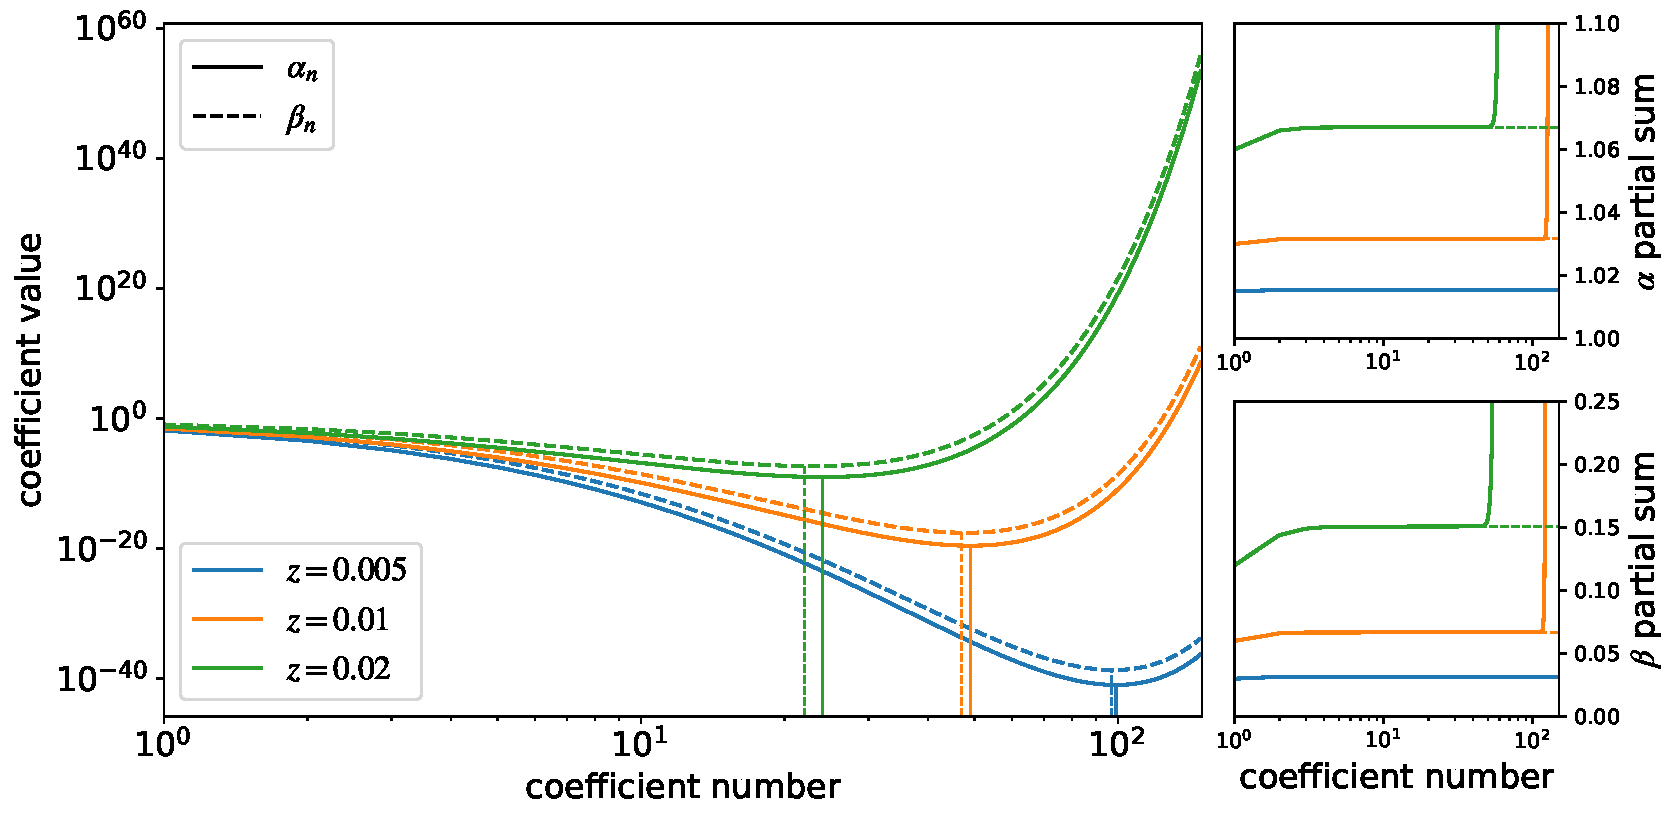
\includegraphics[width=\linewidth]{figures/alpha_beta.pdf}
        \oscaption{alpha_beta}{%
            Asymptotic series expansions for $\alpha$ and $\beta$
            (Equations~\ref{eq:alpha} and \ref{eq:beta}).
            The left panel shows the value of each
            coefficient ($\alpha$: solid, $\beta$: dashed)
            as a function of the index $n$ for three
            different values of $z$. In all cases, the value initially decreases
            with $n$ but eventually diverges to $+\infty$ as $n \rightarrow \infty$.
            The vertical lines indicate the optimal truncation order $N$,
            for which the partial sums yield the best approximation to the
            asymptotic values of the cofficients. The right panels show the
            partial sums evaluated at each order; the value at the optimal
            truncation order is marked with the horizontal dashed lines.
            \label{fig:alpha_beta}
        }
    \end{centering}
\end{figure}
%
This is demonstrated in Figure~\ref{fig:alpha_beta}, which shows the
terms in the summations in Equations~\ref{eq:alpha} and \ref{eq:beta} for
different values of $z$. While the terms initially decrease in magnitude
(left panel), asymptotically approaching a finite value for both
$\alpha$ and $\beta$ (right panels), as the expansion order increases
the terms eventually diverge, leading to infinite values for both
coefficients. Even though the series take longer to diverge for smaller
values of $z$, the divergence occurs for all $z \ne 0$: i.e., the radius
of convergence for both series is zero.

Why is this? Recall the assumption we made when expanding the expectation
integrals in Equations~(\ref{eq:WhereItAllGoesWrong1}), (\ref{eq:WhereItAllGoesWrong2}),
and (\ref{eq:WhereItAllGoesWrong3}): the Taylor expansion converges only for
$\big|\epsilon| < 1$. The quantity $\epsilon$ (Equation~\ref{eq:epsilon})
is indeed small provided the sample mean $\bar{x}$ is close to the GP
mean $\mu$. However, $\epsilon$ is a random variable, equal to
the weighted sum of $K$ standard normal random variables. Because a normal
distribution has infinite support, $\epsilon$ is guaranteed to take on
values greater than unity in the limit that an infinite number of samples
are drawn from the process. In particular, it is guaranteed to take on values
arbitrarily close to unity, in which case the sample mean approaches zero and
the values in the normalized sample diverge.
This reveals a fundamental flaw in our premise:
it is simply not correct to normalize a sample from a Gaussian process by its
mean value, since the resulting covariance is formally infinite.

Nevertheless, if one were to draw a very large number of samples from a normal
distribution with unit mean and small standard deviation,
the probability of drawing a sample with mean close to or smaller than zero
is vanishingly small (for example, for $\sigma \lesssim 0.1$, this probability
is $\lesssim 10^{-22}$).
Any numerical (sampling) estimate of the
covariance matrix of the normalized Gaussian process will therefore yield
a result that asymptotically approaches a finite, consistent value as the
number of samples increases. If it were practical to draw
$\sim 10^{22}$ samples, however, the estimate would eventually diverge, since
some of the normalized samples would have divergent values.

This is the exact same behavior we see in the series solution above.
While the series formally diverges, the finite asymptotic value obtained
by truncating the expansion early can be understood as an estimate of
the covariance of the normalized process \emph{ignoring the divergent
    tails of the distribution}.

In the following sections, we empirically show that this interpretation is
correct, and that the expression for the normalized covariance
(Equation~\ref{eq:SigmaTilde}) is accurate provided $z \ll 1$.

\section{Non-stationarity}

%
\begin{figure}[t!]
    \begin{centering}
        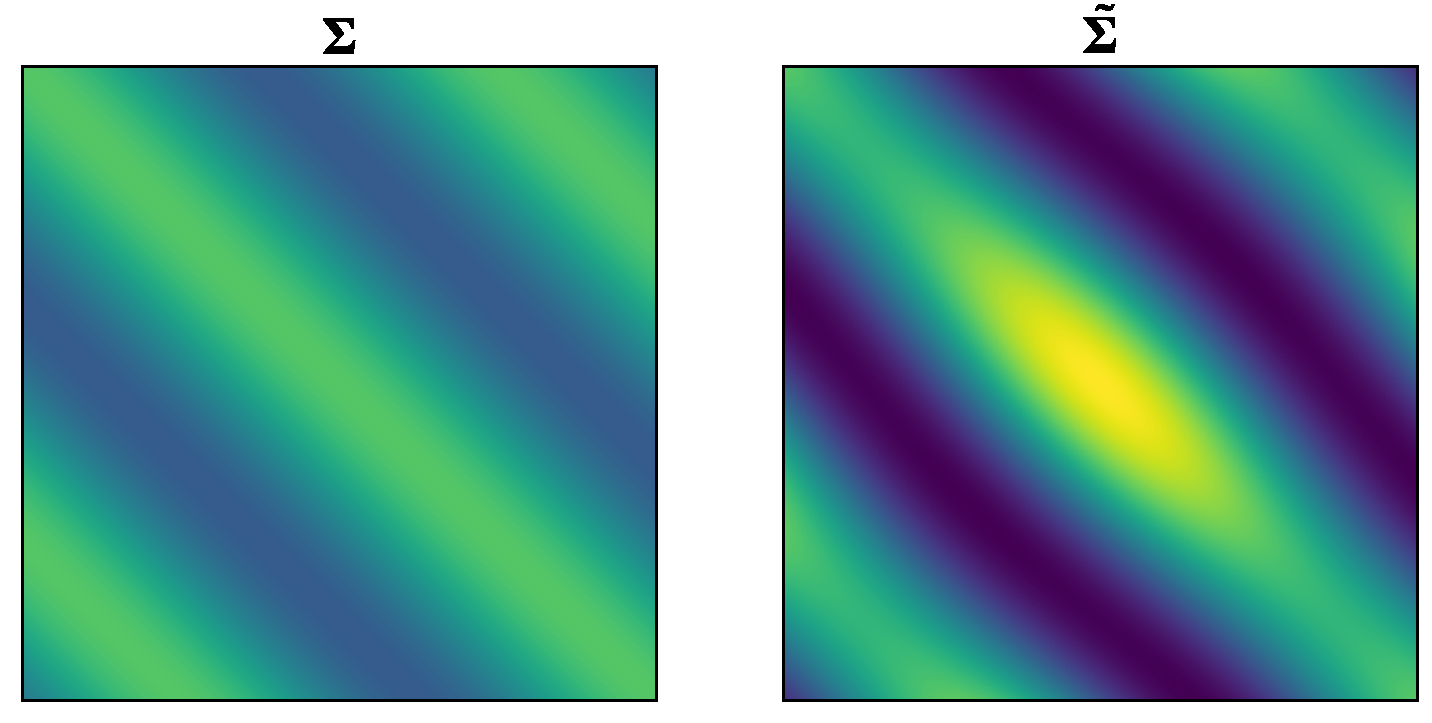
\includegraphics[width=\linewidth]{figures/periodic.pdf}
        \oscaption{periodic}{%
            The covariance matrix corresponding to a periodic kernel
            (left) and the covariance matrix of the corresponding
            normalized process (right).
            \label{fig:periodic}
        }
    \end{centering}
\end{figure}

\ifdefined \includeAppendix

    \clearpage

    \appendix

    \section{Computing $\tilde{\pmb{\Sigma}}$}
    %
    Since the expectation is a linear operator, we can write Equation~(\ref{eq:SigmaTildeExp})
    as
    %
    \begin{align}
        \tilde{\pmb{\Sigma}}
         & =
        \frac{1}{\mu^2}
        \sum\limits_{n=0}^\infty
        (-1)^n (n + 1)
        \,
        \mathbb{E}\left[
            \epsilon^n
            \Bigg(
            \mu^2 \mathbf{j} \, \mathbf{j}^\top
            +
            \mu \, \mathbf{j}\mathbf{u}^\top \mathbf{L}^\top
            +
            \mu \, \mathbf{L} \, \mathbf{u} \, \mathbf{j}^\top
            +
            \mathbf{L} \, \mathbf{u} \, \mathbf{u}^\top \, \mathbf{L}^\top
            \Bigg)
            \right]
        - \mathbf{j} \, \mathbf{j}^\top
        \nonumber \\[0.5em]
         & =
        \sum\limits_{n=0}^\infty
        \frac{(-1)^n}{\mu^{2 + n}}
        \,
        \left(
        \mu^2 \mathbf{P}_n
        +
        \mu \, \mathbf{Q}_n
        +
        \mu \, \mathbf{Q}_n^\top
        +
        \mathbf{R}_n
        \right)
        - \mathbf{j} \, \mathbf{j}^\top
        \quad,
    \end{align}
    %
    where we define the matrices
    %
    \begin{align}
        \mathbf{P}_n & \equiv \frac{(n + 1)}{K^n}\mathbb{E}\left[ \left(\mathbf{j}^\top \mathbf{L} \, \mathbf{u}\right)^n \mathbf{j} \, \mathbf{j}^\top \right]
        \nonumber                                                                                                                                                                                \\[0.5em]
        \mathbf{Q}_n & \equiv \frac{(n + 1)}{K^n}\mathbb{E}\left[ \left(\mathbf{j}^\top \mathbf{L} \, \mathbf{u}\right)^n \mathbf{L} \, \mathbf{u} \, \mathbf{j}^\top \right]
        \nonumber                                                                                                                                                                                \\[0.5em]
        \mathbf{R}_n & \equiv \frac{(n + 1)}{K^n}\mathbb{E}\left[ \left(\mathbf{j}^\top \mathbf{L} \, \mathbf{u}\right)^n \mathbf{L} \, \mathbf{u} \, \mathbf{u}^\top \, \mathbf{L}^\top \right]
        \quad.
    \end{align}
    %
    In order to compute these matrices,
    we will make use of the expression for the
    $n^\mathrm{th}$ moment of the standard normal distribution:
    %
    \begin{align}
        \mathbb{E}\left[ u^n \right] & = g_n
    \end{align}
    %
    for scalar $u \sim \mathcal{N}(0, 1)$, where
    %
    \begin{align}
        g_n
         & =
        \begin{cases}
            \dfrac{n!}{2^\frac{n}{2} \left(\frac{n}{2}\right)!} & n \, \mathrm{even}
            \\
            0                                                   & n \, \mathrm{odd}
            \quad.
        \end{cases}
    \end{align}
    %
    \citep[e.g.,][]{Winkelbauer2012}.
    We can apply this relation to compute expectations
    of products of the components of a random standard normal vector $\mathbf{u}$:
    %
    \begin{align}
        \mathbb{E}\left[u_i \right]                  & = 0
        \\[1em]
        \mathbb{E}\left[u_i u_j\right]               & = g_2
        \\[1em]
        \mathbb{E}\left[u_i u_j u\right]             & = 0
        \\[1em]
        \mathbb{E}\left[u_i u_j u u_l\right]         & =
        g_4 \, \delta_{i, j} \delta_{k, l} \, \delta_{i, k}
        +
        g_2^2 \left(
        \delta_{i, j} \, \delta_{k, l} \, \bar{\delta}_{i, k}
        +
        \delta_{i, k} \, \delta_{j, l} \, \bar{\delta}_{i, j}
        +
        \delta_{i, l} \, \delta_{j, k} \, \bar{\delta}_{i, j}
        \right)
        \\[1em]
        \mathbb{E}\left[u_i u_j u u_l u_m\right]     & = 0
        \\[1em]
        \mathbb{E}\left[u_i u_j u u_l u_m u_n\right] & =
        ...
        \quad,
    \end{align}
    %
    where $\delta$ is the Kronecker delta and $\bar{\delta} \equiv 1 - \delta$.

    \subsection{The $\mathbf{P}$ expectation}

    Let us begin by computing the first several terms in $\mathbf{P}$.
    %
    \begin{align}
        \mathbf{P}_0 & = \mathbb{E}\left[ \mathbf{j} \, \mathbf{j}^\top \right]
        \nonumber                                                               \\
                     & = \mathbf{j} \, \mathbf{j}^\top
    \end{align}
    %
    since $\mathbf{j} \, \mathbf{j}^\top$ is constant. Next,
    %
    \begin{align}
        \mathbf{P}_1 & = \frac{2}{K}\mathbb{E}\left[ \left(\mathbf{j}^\top \mathbf{L} \, \mathbf{u}\right) \mathbf{j} \, \mathbf{j}^\top \right]
        \nonumber                                                                                                                                \\
                     & = \frac{2}{K}\left(\mathbf{j}^\top \mathbf{L} \, \mathbb{E}\left[ \mathbf{u} \right]\right) \mathbf{j} \, \mathbf{j}^\top
        \nonumber                                                                                                                                \\
                     & = \mathbf{0}
    \end{align}
    %
    since $\mathbb{E}\left[ \mathbf{u} \right] = \mathbf{0}$. The next term is
    %
    \begin{align}
        \mathbf{P}_2 & = \frac{3}{K^2}\mathbb{E}\left[ \left(\mathbf{j}^\top \mathbf{L} \, \mathbf{u}\right)^2 \mathbf{j} \, \mathbf{j}^\top \right]
        \nonumber                                                                                                                                                                                   \\
                     & = \frac{3}{K^2}\mathbb{E}\left[\left(\mathbf{j}^\top \mathbf{L} \,  \mathbf{u} \mathbf{u}^\top  \mathbf{L}^\top \, \mathbf{j} \right)  \mathbf{j} \, \mathbf{j}^\top \right]
        \nonumber                                                                                                                                                                                   \\
                     & = \frac{3}{K^2}\left(\mathbf{j}^\top \mathbf{L} \, \mathbb{E}\left[ \mathbf{u} \mathbf{u}^\top \right] \mathbf{L}^\top \, \mathbf{j} \right)  \mathbf{j} \, \mathbf{j}^\top
        \nonumber                                                                                                                                                                                   \\
                     & = \frac{3}{K^2}\left(\mathbf{j}^\top \mathbf{L} \mathbf{L}^\top \, \mathbf{j} \right)  \mathbf{j} \, \mathbf{j}^\top
        \nonumber                                                                                                                                                                                   \\
                     & = \frac{3}{K^2}\mathrm{sum}(\mathbf{\Sigma}) \mathbf{j} \, \mathbf{j}^\top
        \nonumber                                                                                                                                                                                   \\
                     & = 3 \, m \, \mathbf{j} \, \mathbf{j}^\top
    \end{align}
    %
    where $m$ is the average of all entries in $\pmb{\Sigma}$ and
    we made use of the fact that $\mathbb{E}\left[ \mathbf{u} \mathbf{u}^\top\right] = \mathbf{I}$.
    %
    Next,
    %
    \begin{align}
        \mathbf{P}_3 & = \frac{4}{K^3}\mathbb{E}\left[ \left(\mathbf{j}^\top \mathbf{L} \, \mathbf{u}\right)^3 \mathbf{j} \, \mathbf{j}^\top \right]
        \nonumber                                                                                                                                                                                                                               \\
                     & = \frac{4}{K^3}\mathbb{E}\left[\left(\mathbf{j}^\top \mathbf{L} \,  \mathbf{u} \mathbf{u}^\top  \mathbf{L}^\top \, \mathbf{j} \, \mathbf{j}^\top \mathbf{L} \,  \mathbf{u} \right) \mathbf{j} \, \mathbf{j}^\top \right]
        \nonumber                                                                                                                                                                                                                               \\
                     & = \frac{4}{K^3}\left(\mathbf{j}^\top \mathbf{L} \,  \mathbb{E}\left[\mathbf{u} \mathbf{u}^\top  \mathbf{L}^\top \, \mathbf{j} \, \mathbf{j}^\top \mathbf{L} \,  \mathbf{u}\right] \right) \mathbf{j} \, \mathbf{j}^\top
        \nonumber                                                                                                                                                                                                                               \\
                     & = \mathbf{0}
    \end{align}
    %
    where we made use of the fact that we may write the component at index $i$ of the vector within the expectation in the next-to-last line
    as
    \begin{align}
        \mathbb{E}\left[\mathbf{u} \mathbf{u}^\top  \mathbf{L}^\top \, \mathbf{j} \, \mathbf{j}^\top \mathbf{L} \,  \mathbf{u}\right]_{i} = \sum\limits_{k,l}(\mathbf{L}^\top \mathbf{j} \, \mathbf{j}^\top \mathbf{L})_{kl} u_i u u_l = 0
        \quad,
        \nonumber
    \end{align}
    %
    which is zero since it is the product of an odd number of random normal variables.
    Finally,
    %
    \begin{align}
        \mathbf{P}_4 & = \frac{5}{K^4}\mathbb{E}\left[ \left(\mathbf{j}^\top \mathbf{L} \, \mathbf{u}\right)^4 \mathbf{j} \, \mathbf{j}^\top \right]
        \nonumber                                                                                                                                                                                                                                                                                 \\
                     & = \frac{5}{K^4}\mathbb{E}\left[\left(\mathbf{j}^\top \mathbf{L} \,  \mathbf{u} \mathbf{u}^\top  \mathbf{L}^\top \, \mathbf{j} \, \mathbf{j}^\top \mathbf{L} \,  \mathbf{u} \, \mathbf{u}^\top  \mathbf{L}^\top \, \mathbf{j} \right) \mathbf{j} \, \mathbf{j}^\top \right]
        \nonumber                                                                                                                                                                                                                                                                                 \\
                     & = \frac{5}{K^4}\left(\mathbf{j}^\top \mathbf{L} \, \mathbf{E} \, \mathbf{L}^\top \, \mathbf{j} \right) \mathbf{j} \, \mathbf{j}^\top
        \quad,
    \end{align}
    %
    where we define
    %
    \begin{align}
        \mathbf{E} \equiv \mathbb{E}\left[ \mathbf{u} \mathbf{u}^\top  \mathbf{A} \,  \mathbf{u} \mathbf{u}^\top \right]
    \end{align}
    %
    and
    %
    \begin{align}
        \mathbf{A} \equiv \mathbf{L}^\top \, \mathbf{j} \, \mathbf{j}^\top \, \mathbf{L}
        \quad.
    \end{align}
    %
    The components of this matrix are
    %
    \begin{align}
        E_{ij} & =
        \sum\limits_{k,l}A_{kl} \mathbb{E}(u_i u_j u u_l)
        \nonumber  \\
               & =
        \sum\limits_{k,l}A_{kl}
        \Big(
        g_4 \, \delta_{i, j} \, \delta_{k, l} \, \delta_{i, k}
        +
        g_2^2 \big(
            \delta_{i, j} \, \delta_{k, l} \, \bar{\delta}_{i, k}
            +
            \delta_{i, k} \, \delta_{j, l} \, \bar{\delta}_{i, j}
            +
            \delta_{i, l} \, \delta_{j, k} \, \bar{\delta}_{i, j}
            \big)
        \Big)
        \nonumber  \\
               & =
        2 A_{ij} + \sum\limits A_{kk}
        \quad,
    \end{align}
    %
    where we used the fact that $\mathbf{A} = \mathbf{A}^\top$. We may thus write
    %
    \begin{align}
        \mathbf{E} & =
        2 \, \mathbf{A} + \mathrm{tr}(\mathbf{A}) \mathbf{I}
        \nonumber      \\
                   & =
        2 \, \mathbf{L}^\top \, \mathbf{j} \, \mathbf{j}^\top \, \mathbf{L} + \mathrm{sum}(\pmb{\Sigma}) \mathbf{I}
        \quad.
    \end{align}
    %
    Inserting this back into the expression for $\mathbf{P}_4$, we obtain
    %
    \begin{align}
        \mathbf{P}_4 & =
        \frac{5}{K^4}
        \bigg(
        2 \, \big(\mathbf{j}^\top \mathbf{L} \, \mathbf{L}^\top \, \mathbf{j} \, \mathbf{j}^\top \, \mathbf{L} \, \mathbf{L}^\top \, \mathbf{j} \big)
        +
        \mathrm{sum}(\pmb{\Sigma}) \big(\mathbf{j}^\top \mathbf{L} \, \mathbf{L}^\top \, \mathbf{j} \big)
        \bigg) \mathbf{j} \, \mathbf{j}^\top
        \nonumber        \\
                     & =
        3 \, m^2 \mathbf{j} \, \mathbf{j}^\top
        \quad.
    \end{align}
    %
    The general term in this sequence is
    %
    \begin{align}
        \mathbf{P}_n & =
        \mathbf{j} \, \mathbf{j}^\top
        \begin{cases}
            0                            & n \, \mathrm{odd}
            \\
            g_n (n + 1) \, m^\frac{n}{2} & n \, \mathrm{even}
            \quad.
        \end{cases}
    \end{align}
    %


    \subsection{The $\mathbf{Q}$ expectation}
    %
    Let us again compute the first several terms of this expectation matrix.
    %
    \begin{align}
        \mathbf{Q}_0 & = \mathbb{E}\left[ \mathbf{L} \, \mathbf{u} \, \mathbf{j}^\top \right]
        \nonumber                                                                                                                                              \\
                     & = \mathbf{L} \, \mathbb{E}\left[  \mathbf{u} \right] \, \mathbf{j}^\top
        \nonumber                                                                                                                                              \\
                     & = \mathbf{0}
        %
        \\[1em]
        %
        \mathbf{Q}_1 & = \frac{1}{K}\mathbb{E}\left[ \left(\mathbf{j}^\top \mathbf{L} \, \mathbf{u}\right) \mathbf{L} \, \mathbf{u} \, \mathbf{j}^\top \right]
        \nonumber                                                                                                                                              \\
                     & = \frac{1}{K}\mathbb{E}\left[ \left(\mathbf{j}^\top \mathbf{L} \, \mathbf{u}\right) \mathbf{L} \, \mathbf{u} \right] \, \mathbf{j}^\top
        \nonumber                                                                                                                                              \\
                     & = \frac{1}{K}\mathbb{E}\left[ \mathbf{L} \, \mathbf{u} (\mathbf{u}^\top \mathbf{L}^\top \mathbf{j}) \right] \, \mathbf{j}^\top
        \nonumber                                                                                                                                              \\
                     & = \frac{1}{K}\mathbb{E}\left[ \mathbf{L} \, \mathbf{u} \mathbf{u}^\top \mathbf{L}^\top  \right] \, \mathbf{j} \, \mathbf{j}^\top
        \nonumber                                                                                                                                              \\
                     & = \frac{1}{K}\mathbf{L} \, \mathbb{E}\left[  \mathbf{u} \mathbf{u}^\top   \right]  \, \mathbf{L}^\top \mathbf{j} \, \mathbf{j}^\top
        \nonumber                                                                                                                                              \\
                     & = \frac{1}{K}\mathbf{L} \, \mathbf{L}^\top \mathbf{j} \, \mathbf{j}^\top
        \nonumber                                                                                                                                              \\
                     & = \frac{1}{K}\pmb{\Sigma} \, \mathbf{j} \, \mathbf{j}^\top
    \end{align}
    %
    where we made liberal use of the fact that $\left(\mathbf{j}^\top \mathbf{L} \, \mathbf{u}\right)$ is a scalar. Continuing,
    %
    \begin{align}
        \mathbf{Q}_2 & = \frac{2}{K^2}\mathbb{E}\left[ \left(\mathbf{j}^\top \mathbf{L} \, \mathbf{u}\right)^2 \mathbf{L} \, \mathbf{u} \, \mathbf{j}^\top \right]
        \nonumber                                                                                                                                                                                    \\
                     & =  \frac{2}{K^2}\mathbb{E}\left[ \mathbf{L} \, \mathbf{u} \, (\mathbf{j}^\top \mathbf{L} \, \mathbf{u}) (\mathbf{u}^\top \mathbf{L}^\top \mathbf{j}) \mathbf{j}^\top \right]
        \nonumber                                                                                                                                                                                    \\
                     & = \frac{2}{K^2}\mathbf{L} \, \mathbb{E}\left[ \mathbf{u} \, \mathbf{j}^\top \mathbf{L} \, \mathbf{u} \mathbf{u}^\top \right] \, \mathbf{L}^\top \mathbf{j} \, \mathbf{j}^\top
        \nonumber                                                                                                                                                                                    \\
                     & = \mathbf{0}
    \end{align}
    %
    since again the components of the expectation in the next-to-last line involve products of three standard normal random variables.
    Next,
    \begin{align}
        \mathbf{Q}_3 & = \frac{3}{K^3}\mathbb{E}\left[ \left(\mathbf{j}^\top \mathbf{L} \, \mathbf{u}\right)^3 \mathbf{L} \, \mathbf{u} \, \mathbf{j}^\top \right]
        \nonumber                                                                                                                                                  \\
                     & = \xxx{...}
        \nonumber                                                                                                                                                  \\
                     & =
        \frac{3}{K^3}\mathbf{e} \, \mathbf{j}^\top
    \end{align}
    %
    % 3 \, \pmb{\Sigma} \, \mathbf{j} \, \mathbf{j}^\top \, \pmb{\Sigma} \, \mathbf{j} \, \mathbf{j}^\top
    %
    where we define
    %
    \begin{align}
        \mathbf{e} \equiv \mathbb{E}\left[
            \left(
            \mathbf{v}^\top \mathbf{u} \mathbf{u}^\top \mathbf{v}
            \mathbf{v}^\top \mathbf{u}
            \right)
            \mathbf{L} \mathbf{u}
            \right]
    \end{align}
    %
    and
    %
    \begin{align}
        \mathbf{v} \equiv \mathbf{L}^\top \, \mathbf{j}
        \quad.
    \end{align}
    %
    The components of $\mathbf{e}$ are given by
    %
    \begin{align}
        e_{i} & =
        \sum\limits_{j,k,l,m}L_{ij} v v_l v_m \mathbb{E}(u_j u u_l u_m)
        \nonumber \\
              & =
        \sum\limits_{j,k,l,m}L_{ij} v v_l v_m
        \Big(
        g_4 \, \delta_{j, k} \, \delta_{l, m} \, \delta_{j, l}
        +
        g_2^2 \big(
            \delta_{j, k} \, \delta_{l, m} \, \bar{\delta}_{j, l}
            +
            \delta_{j, l} \, \delta_{k, m} \, \bar{\delta}_{j, k}
            +
            \delta_{j, m} \, \delta_{k, l} \, \bar{\delta}_{j, k}
            \big)
        \Big)
        \nonumber \\
              & =
        \xxx{...}
    \end{align}
    %
    We may thus write
    %
    \begin{align}
        \mathbf{e} & = 3 \, \pmb{\Sigma} \, \mathbf{j} \, \mathbf{j}^\top \, \pmb{\Sigma} \, \mathbf{j}
        \quad.
    \end{align}
    %
    Inserting this back into the expression for $\mathbf{Q}_3$, we obtain
    %
    \begin{align}
        \mathbf{Q}_3 & =
        \frac{9}{K^3} \, (\pmb{\Sigma} \, \mathbf{j} \, \mathbf{j}^\top)^2
    \end{align}
    %
    Based on this pattern, the general term in $\mathbf{Q}$ is
    %
    \begin{align}
        \mathbf{Q}_n & =
        \begin{cases}
            \mathbf{0}                                                                                    & n \, \mathrm{even}
            \\
            \frac{(n + 1)g_{n+1}}{K^n} \, (\pmb{\Sigma} \, \mathbf{j} \, \mathbf{j}^\top)^\frac{n + 1}{2} & n \, \mathrm{odd}
            \quad.
        \end{cases}
    \end{align}

    \subsection{The $\mathbf{R}$ expectation}
    %
    The first several terms in $\mathbf{R}$ are given by
    %
    \setlength{\abovedisplayskip}{1em}
    \begin{align}
        \mathbf{R}_0 & = \mathbb{E}\left[ \mathbf{L} \, \mathbf{u} \, \mathbf{u}^\top \mathbf{L}^\top \right]
        \nonumber                                                                                                                                                              \\
                     & = \mathbf{L} \, \mathbb{E}\left[  \mathbf{u} \, \mathbf{u}^\top \right] \, \mathbf{L}^\top
        \nonumber                                                                                                                                                              \\
                     & = \pmb{\Sigma}
        %
        \\[1em]
        %
        \mathbf{R}_1 & = \frac{1}{K}\mathbb{E}\left[ \left(\mathbf{j}^\top \mathbf{L} \, \mathbf{u}\right) \mathbf{L} \, \mathbf{u} \, \mathbf{u}^\top \mathbf{L}^\top \right]
        \nonumber                                                                                                                                                              \\
                     & = \mathbf{0}
        %
    \end{align}
    %
    since its elements are all products of three standard normal random variables. Next,
    %
    \begin{align}
        %
        \mathbf{R}_2 & = \mathbb{E}\left[ \left(\mathbf{j}^\top \mathbf{L} \, \mathbf{u}\right)^2 \mathbf{L} \, \mathbf{u} \, \mathbf{u}^\top \mathbf{L}^\top \right]
        \nonumber                                                                                                                                                     \\
                     & = \xxx{...}
        \nonumber                                                                                                                                                     \\
                     & = 2 \pmb{\Sigma} \mathbf{j} \, \mathbf{j}^\top \pmb{\Sigma} + \mathrm{sum}(\pmb{\Sigma}) \pmb{\Sigma}
    \end{align}
    %
    \xxx{By trial and error, I found that}
    %
    \begin{align}
        %
        \mathbf{R}_4 & = \frac{5}{K^4}\mathbb{E}\left[ \left(\mathbf{j}^\top \mathbf{L} \, \mathbf{u}\right)^4 \mathbf{L} \, \mathbf{u} \, \mathbf{u}^\top \mathbf{L}^\top \right]
        \nonumber                                                                                                                                                                  \\
                     & = \xxx{...}
        \nonumber                                                                                                                                                                  \\
                     & = \frac{5}{K^4} \Big( 12 (\pmb{\Sigma} \mathbf{j} \, \mathbf{j}^\top)^2 \pmb{\Sigma} + 3 \, \mathrm{sum}(\pmb{\Sigma})^2 \pmb{\Sigma} \Big)
    \end{align}
    %
    Based on this pattern, the general term in $\mathbf{R}$ is
    %
    \begin{align}
        \mathbf{R}_n & =
        \begin{cases}
            \mathbf{0}                                                                                                                                           & n \, \mathrm{odd}
            \\
            \frac{n (n + 1) g_{n}}{K^n} \, (\pmb{\Sigma} \, \mathbf{j} \, \mathbf{j}^\top)^\frac{n}{2}\pmb{\Sigma} + (n + 1) g_{n} \, m^\frac{n}{2} \pmb{\Sigma} & n \, \mathrm{even}
            \quad.
        \end{cases}
    \end{align}

    \subsection{The final result}
    Inserting the matrices $\mathbf{P}$, $\mathbf{Q}$, and $\mathbf{R}$ into the expression
    for $\tilde{\pmb{\Sigma}}$ and rearranging,
    we obtain
    %
    \begin{align}
        \tilde{\pmb{\Sigma}}
         & =
        \frac{1}{\mu^2} \pmb{\Sigma}
        +
        \frac{1}{\mu^2}
        \sum\limits_{n=1}^\infty
        \frac{(-1)^n(n + 1)}{\mu^{n}}
        \,
        \bigg[
            g_n \, m^\frac{n}{2} \, (\pmb{\Sigma} + \mu^2\mathbf{j} \, \mathbf{j}^\top)
            \, +
            \nonumber                 \\[0.5em]
         & \phantom{XXXXXXXXXXXXXXX.}
        K g_{n+1} \mu  \,
        \left(
        \left(\pmb{\Sigma} \, \frac{\mathbf{j} \, \mathbf{j}^\top}{K^2}\right)^\frac{n + 1}{2}
        +
        \left(\frac{\mathbf{j} \, \mathbf{j}^\top}{K^2} \, \pmb{\Sigma}\right)^\frac{n + 1}{2}
        \right)
        \, +
        \nonumber                     \\[0.5em]
         & \phantom{XXXXXXXXXXXXXXX.}
        n g_n \, \left(\pmb{\Sigma} \, \frac{\mathbf{j} \, \mathbf{j}^\top}{K^2}\right)^\frac{n}{2}\pmb{\Sigma}
        \bigg]
        \quad.
    \end{align}

\else
\fi

\bibliography{bib}

\end{document}